\documentclass[12pt]{article}
\usepackage[margin=3cm]{geometry}
\usepackage[portuguese]{babel}
\usepackage[utf8]{inputenc}
\usepackage{fancyhdr}
\usepackage{hyperref}
\usepackage{indentfirst}
\usepackage[pdftex]{graphicx}
\usepackage{siunitx}

\urlstyle{same}
\pagestyle{fancy}
\fancyhf{}
\author{
	Grupo: al024\\Alunos: António Coelho (ist195535) e Gustavo Aguiar (ist195587)
}
\title{\vspace{-2cm}Relatório 2º Projeto ASA 2020/2021}
\date{}
\hypersetup{
    colorlinks=true,
    linkcolor=black,
    filecolor=black,      
    urlcolor=cyan,
}
\fancyfoot[C]{\thepage}

\begin{document}
\maketitle
\section{Descrição do Problema e da Solução}
Pelo enunciado, temos que o pretendido é $min$\{$\sum_{i\in{P_{x}}}$X$_{i}$ + $\sum_{i\in{P_{y}}}$Y$_{i}$ + $\sum_{(i, j)\in{P_{x} \times P_{y}}}$c$_{ij}$\}. Assim, por definição, este problema trata-se de um corte de capacidade mínima, pelo que com base no Teorema de Fluxo Máximo Corte Mínimo, modelámo-lo como um de rede de fluxo, onde a fonte e o sumidouro correspondem aos processadores X e Y, respetivamente, e os restantes vértices aos $n$ processos do programa.
Para além disso, sabendo que ($\sum_{i\in{P_{x}}}$$X_{i}$ + $\sum_{i\in{P_{y}}}$$Y_{i}$) $\in{O(n)}$, temos que $\left|f^{*}\right|$ $\in{O(\left|V\right|)}$. Justifica-se assim usar um algoritmo de caminhos de aumento, baseado no método de \emph{Ford-Fulkerson}, sendo esses determinados por uma \emph{BFS} - \textbf{Algoritmo de \emph{Edmonds-Karp}}.

Assim, como auxílio de resolução dos problemas encontrados utilizaram-se as seguintes referências:
\begin{itemize}
\item\href{https://brilliant.org/wiki/edmonds-karp-algorithm/}{Análise teórica do algoritmo de \emph{Edmonds-Karp}}
\item\href{https://www.geeksforgeeks.org/ford-fulkerson-algorithm-for-maximum-flow-problem/}{Implementação do algoritmo de \emph{Edmonds-Karp} para determinar o fluxo máximo}
\end{itemize}
 
 \section{Análise Teórica}
 A representação da rede residual em memória foi feita com recurso a uma matriz de adjacências - complexidade de espaço $\Theta{(V^2)}$ - justificada pela bidirecionalidade dos arcos correspondentes aos custos inter-processos e pelo acesso O(1) às capacidades dos arcos na rede residual no decorrer do algoritmo.

A solução visada para a resolução dos problemas apresentados consiste em 2 etapas: ler a rede de fluxo de \emph{input} (\underline{1}) e computar o fluxo máximo com recurso ao algoritmo de \emph{Edmonds-Karp}(\underline{2}).

Para (\underline{1}) - leitura de \emph{input} - usando \texttt{scanf}, ler os dados de entrada dentro de dois ciclos ($n$ e $k$) a dependerem linearmente e quadraticamente de V para os custos entre os processos e os processadores e entre processos, respetivamente. Mais concretamente, $\Theta{(V - 2)}$ = O(V) para o primeiro ciclo e O($\frac{(V-2)(V-3)}{2}$) = O(V$^2$) para o segundo.

Para (\underline{2}) - aplicar o algoritmo de \emph{Edmonds-Karp} na rede de fluxo - enquanto houver caminhos de aumento (o que se verifica em O($VE$) vezes) aplica-se a \emph{BFS}(O(V$^2$), uma vez que se trata de uma matriz de adjacências) para encontrar entre esses o mais curto em número de arcos - distância de \emph{Edmonds-Karp} mínima. Existindo um, determina-se a sua capacidade crítica por \emph{backtrack} (que é O(V)) e o fluxo máximo é incrementado esse valor. No total tem-se O(VE(V$^2$+V)) = O(EV$^3$).

Por fim, como a complexidade de (\underline{2}) domina a de (\underline{1}), tem-se que a solução geral aos problemas apresentados $\in{\textbf{O(EV$^3$)}}$.

\section{Avaliação Experimental dos Resultados}
Para a devida análise do algoritmo implementado, utilizou-se um computador com processador \emph{Intel Core i5 Quad-Core} a \SI{1,4}{GHz}, com \SI{8}{GB} de memória RAM, com o sistema operativo \emph{macOS Big Sur}.

Utilizou-se a ferramenta \texttt{gen2procs} fornecida pelo corpo docente para gerar redes de fluxo com capacidade por arco não superior a 15 – mostra-se irrelevante utilizar capacidades muitos superiores uma vez que a solução apresentada tem complexidade independente desse valor - e número de vértices entre 102 e 1602 aumentando de 100 em 100, perfazendo um tamanho de grafo até à ordem de grandeza $10^6$. Com o intuito de cronometrar o desempenho do algoritmo implementado utilizou-se a chamada de sistema \texttt{time} para o programa a correr sobre as tais redes geradas.

\begin{center}
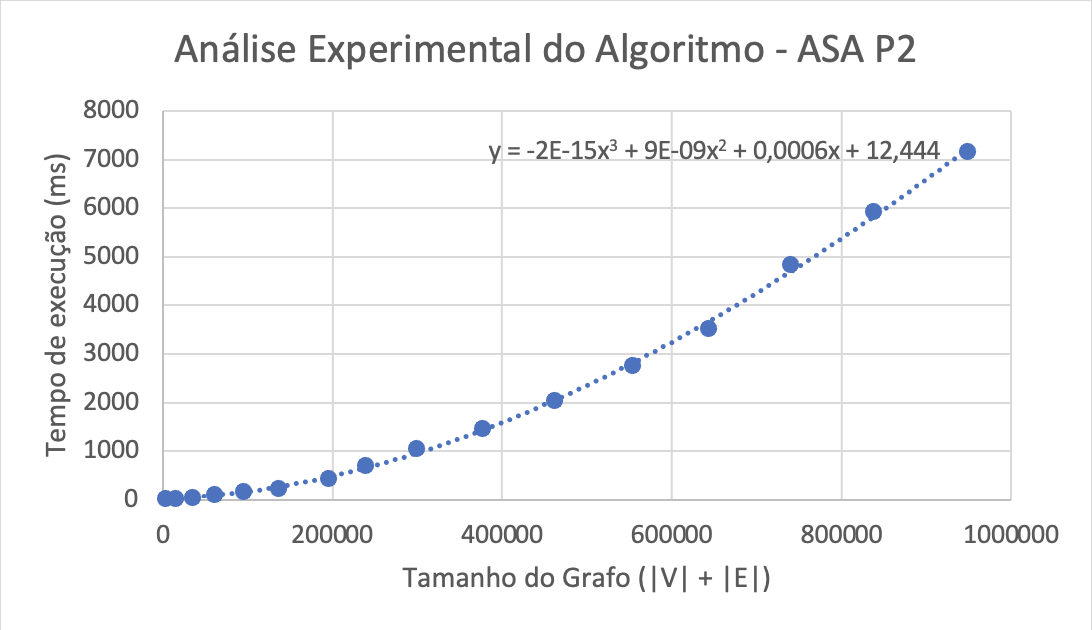
\includegraphics[width=\linewidth]{reglinear.png}
\end{center}

Por fim, registaram-se os valores obtidos da testagem e ajustou-se uma regressão polinomial de ordem 3 que demonstra, experimentalmente, a veracidade da complexidade do algoritmo esperada teoricamente. Como $\left|E\right|$ $\gg$ $\left|V\right|$, vemos que o tempo de execução está proximamemente relacionado com $\left|V^3\right|$, pelo que podemos concluir que o tempo de execução está proximamente relacionado com  $\textbf{O(EV$^3$)}$.

\end{document}